\chapter{Introducción}
\label{cap:Introduccion}

Este capítulo aborda la motivación del trabajo. Se trata de señalar la necesidad que lo origina, su actualidad y pertinencia. Puede incluir también un estado de la cuestión (o estado del arte) en el que se revisen estudios o desarrollos previos, así como en qué medida sirven de base al trabajo que se presenta.

En este capítulo se debería introducir el \emph{contexto disciplinar y tecnológico} en el que se desarrolla el trabajo de modo que entienda con facilidad su ámbito y alcance. Puesto que un TFG no tiene que ser necesariamente un trabajo con aportes novedosos u originales, solo es necesario la inclusión de \emph{estado del arte} cuando este contribuya a aclarar aspectos clave del TFG o se desee justificar la originalidad del trabajo realizado.

Este capítulo suele finalizar indicando la estructura (capítulos) del documento y el contenido de cada una de las partes en que se divide. Por tanto, las secciones que suelen acompañar este capítulo son:
\begin{enumerate}
    \item \textbf{Motivación}. Responde a la pregunta sobre la necesidad o pertinencia del trabajo.
    \item \textbf{Objetivo}. Determina de modo claro el propósito del trabajo descrito que se puede desglosar en subobjetivos cuando el objetivo principal se descompone en módulos o componentes. Es muy importante definir el objetivo de modo apropiado. El capítulo~\ref{cap:Objetivo} de esta guía explica cómo definir el objetivo del trabajo.
    \item \textbf{Antecedentes} o \emph{Contexto disciplinar/tecnológico}. También se puede denominar \emph{Estado del Arte} cuando se trata de comentar trabajos relacionados que han abordado la cuestión u objetivo planteado.
    \item \textbf{Estructura del documento}. Donde se explica de modo conciso la estructura del documento.
\end{enumerate}


\section{Redacción de la memoria}
Durante la realización de la memoria del TFG es muy importante respetar la guía de estilo de la institución~\cite{esi19}. Por tanto, el empleo de plantillas para un sistema de procesamiento de textos (p.~ej., Word o \LaTeX) puede requerir su adaptación cuando la plantilla mencionada no haya sido suministrada por la institución a la que se dirige el trabajo.

Para redactar un trabajo académico de modo efectivo se recomienda seguir pautas para obtener un resultado final claro y de lectura fácil, como las expuestas en el blog de Leonor Zozaya~\cite{zozaya17} o el apartado de comunicación eficaz del departamento de Legua y Estilo de la UOC~\cite{uoc}.

A la hora de redactar el texto se debe poner especial atención para evitar el plagio respetando los derechos de propiedad intelectual~\cite{uc3m21}. En particular, merece gran atención la inclusión de gráficos e imágenes procedentes de Internet que no sean de elaboración propia. En este sentido se sugiere la consulta del manual de la Universidad de Cantabria. Dicho documento explica de modo conciso cómo incluir imágenes en un trabajo académico de modo apropiado~\cite{unican18}.

A continuación en esta plantilla se muestran ejemplos de elementos de organización del texto en un documento preparado con \LaTeX{}. Todos estos ejemplos se explican en detalle durante el curso de \LaTeX{}~\cite{salido10}. Todos ellos, así como los recogidos en varias obras de referencia, se pueden emplear para adaptar este documento a las necesidades particulares de los estudiantes \cite{lamport94,grat99,cascales03,mittelbach04,grat07,goos07,wikibookLaTex10}. Entre las obras de consulta disponibles sobre \LaTeX{} se recomienda el uso de las obras gratuitas en español~\cite{oetiker14,borbon21} y las guías disponibles en la página web de \href{https://es.overleaf.com/learn}{Overleaf} (en inglés).




\subsection{Organización de información}
El contenido del trabajo final de estudios se organiza en capítulos que se subdividen en secciones. Con \LaTeX{} este tipo de organización se realiza de modo inmediato mediante la generación automática de los estilos correspondientes a los títulos de cada sección y su inclusión en la tabla de contenidos.

En \LaTeX{}, los ajustes relativos a la generación del formato y estilos asociados a secciones del documento se realizan con el paquete \texttt{titlesec} empleado en esta plantilla.

En las secciones siguientes se comenta la inclusión con \LaTeX{} de distintos elementos de organización de información junto a ejemplos que facilitan su  utilización en la memoria del trabajo.




\subsubsection{Listas}
\label{sec:ejListas}
Existen dos tipos de listas: enumeraciones y listas con viñetas. En el primer tipo los elementos de la lista se preceden de una clave numérica o alfabética, mientras que en el segundo tipo se emplea una viñeta. En ambos casos los elementos se pueden anidar para crear una jerarquía entre ellos. En \LaTeX{} se recomienda la inclusión del paquete \texttt{enumitem} que permite personalizar fácilmente las listas de un documento. A continuación se muestran algunos ejemplos:


\noindent Ejemplo de lista con viñetas personalizadas. 
% Ejemplo: Lista con bullets especiales
% ============
\begin{itemize}
	\item pera
	\item[\ding{43}] manzana % Particularización de viñeta
	\item[\faAward] naranja
\end{itemize}


\noindent Ejemplo de lista condensada con separación mínima, en varias columnas y configuración de la etiqueta.
% Ejemplo: Listas en varias columnas
% ============
\begin{multicols}{2} % El parámetro es el número de columnas de la lista
	\begin{enumerate}[(1),noitemsep]
		\item pera
		\item manzana
		\item naranja
		\item patata
		\item calabaza
		\item fresa
	\end{enumerate}
\end{multicols}





\subsubsection{Ecuaciones matemáticas}
Para escribir ecuaciones matemáticas con \LaTeX{} se recomienda incluir los paquetes siguientes en el documento: \texttt{amsmath}, \texttt{amsfonts}, \texttt{amssymb}. 

La composición de ecuaciones requiere el uso de comandos especializados. Por tanto, para facilitar dicha tarea se aconseja el empleo de programas especializados como \textsf{MathType} o asistentes como el incluido en editores como \TeX studio\footnote{\url{https://www.texstudio.org/}} o herramientas en línea.\footnote{\url{https://latex.codecogs.com/},  \url{http://www.sciweavers.org/free-online-latex-equation-editor}} Es muy sencillo incluir fórmulas matemáticas sencillas en el mismo texto en el que se escribe. Por ejemplo, $h^{2}=a^{2}+b^{2}$ que podría ser la ecuación representativa del teorema de Pitágoras (ver también ec.~\ref{eq:pitagoras}).

Las fórmulas también se pueden separar del texto para que aparezcan destacadas, así:

% Ejemplo: Ecuación no numerada
% ============
\[
c^2  = \int {\left( {a^2  + b^2} \right)}  \cdot dx
\]

Pero si se desea, las ecuaciones pueden ser numeradas de forma automática e incluso utilizar referencias cruzadas a ellas:

% Ejemplo: Ec. numerada. (con código para edición con MathType)
% ============
% MathType!MTEF!2!1!+-
% feqaeaartrvr0aaatCvAUfeBSjuyZL2yd9gzLbvyNv2CaerbuLwBLn
% hiov2DGi1BTfMBaeXatLxBI9gBaebbnrfifHhDYfgasaacH8srps0l
% bbf9q8WrFfeuY-Hhbbf9v8qqaqFr0xc9pk0xbba9q8WqFfea0-yr0R
% Yxir-Jbba9q8aq0-yq-He9q8qqQ8frFve9Fve9Ff0dmeaabaqaciGa
% caGaaeqabaaaamaaaOqaaiaadogadaahaaWcbeqaaiaaikdaaaGccq
% GH9aqpcaWGHbWaaWbaaSqabeaacaaIYaaaaOGaey4kaSIaamOyamaa
% CaaaleqabaGaaGOmaaaaaaa!3910!
\begin{equation} \label{eq:pitagoras}
	h^{2}=b^{2} + c^{2}
\end{equation}





\subsubsection{Tablas}
\label{sec:tablas}
A continuación se incluyen algunos ejemplos de tablas elaboradas con 
\LaTeX{} mediante el empleo de paquetes dedicados. Para la realización de tablas más complejas se recomienda la consulta de \cite{borbon21} y el empleo de asistentes o herramientas en línea.\footnote{\url{https://www.tablesgenerator.com/}}

Se debe observar que el título de las tablas se ubica en la parte superior de la tabla. Puesto que el contenido de la tabla es texto, tiene sentido leer primero el título para contextualizar el contenido de la tabla antes de su lectura.

% Ejemplo: Tabla con macro \cline
% ==========
\begin{table}[H]%
	\centering
	\caption{Ejemplo de uso de la macro \texttt{cline}}
	\label{tab:cline}
	\begin{tabular}[t]{|r|l|}
		\hline
		7C0 & hexadecimal \\[1cm] % Ejemplo de separación fijada entre líneas
		3700 & octal \\ \cline{2-2}
		11111000000 & binario \\
		\hline \hline
		1984 & decimal \\
		\hline
	\end{tabular}
\end{table}


\noindent Ejemplo de tabla en la que se 
controla el ancho de la celda.

% Ejemplo: Ejemplo de tabla con control de la anchura de celda.
% ==========
\begin{table}[H]%
	\centering
	\caption{Ejemplo de tabla con especificación de anchura de columna}
	\label{tab:anchura}
	\begin{tabular}{ | l | l | l | p{5cm} |}
		\hline
		Día & Temp Mín (\textdegree C) & Temp Máx (\textdegree C) & Previsión \\ \hline
		Lunes & 11 & 22 & Día claro y muy soleado. Sin embargo, la brisa de la tarde puede hacer que las temperaturas desciendan \\ \hline
		Martes & 9 & 19 & Nuboso con chubascos en muchas regiones. En Cataluña claro con posibilidad de bancos nubosos al norte de la región \\ \hline
		Miércoles & 10 & 21 & La lluvia continuará por la mañana, pero las 
		condiciones climáticas mejorarán considerablemente por la tarde\\
		\hline
	\end{tabular}
\end{table}






\newpage % NOTA: Observa el efecto del salto de página
\subsubsection{Figuras}
A diferencia de lo que sucede en las tablas, el título de las figuras aparece en la parte inferior de estas. Para la inclusión de las figuras se debe tener en cuenta que su contenido se encuentra en un fichero individual con el formato y resolución apropiados para garantizar la calidad del resultado final.

En esta sección se añaden ejemplos de muestra para la inclusión de 
figuras simples y otras compuestas de subfiguras mediante el empleo del paquete \texttt{subcaption}.

% Ejemplo: Ejemplo de inclusión de figura
% ============
\begin{figure}[H] % Figura fijada en el punto de inclusión (package float)
	\centering
	\includegraphics[width=0.7\linewidth]{./figs/clockCR}
	\caption[Ejemplo de figura]{Fotografía a color 
	(Fuente: J. Salido, CC BY-NC-ND)}
	\label{fig:ejFigure}
\end{figure}


\noindent Ejemplo de figura compuesta por dos subfiguras incluidas mediante paquete \texttt{subcaption}. A través del uso de etiquetas (\texttt{\textbackslash label}) es posible incluir referencias cruzadas a subfiguras como la fotografía en blanco y negro de la Fig.~\ref{fig:fotoBW}.


% Ejemplo: Ejemplo de inclusión de subfiguras
% ============
\begin{figure}[H] % Figura fijada en el punto de inclusión (package float)
	\centering
	\begin{subfigure}[b]{0.4\linewidth}
		\centering
		\includegraphics[width=0.8\linewidth]{./figs/clockCR}
		\caption{Fotografía a color}\label{fig:fotocolor}
	\end{subfigure} 
	\begin{subfigure}[b]{0.4\linewidth}
		\centering
		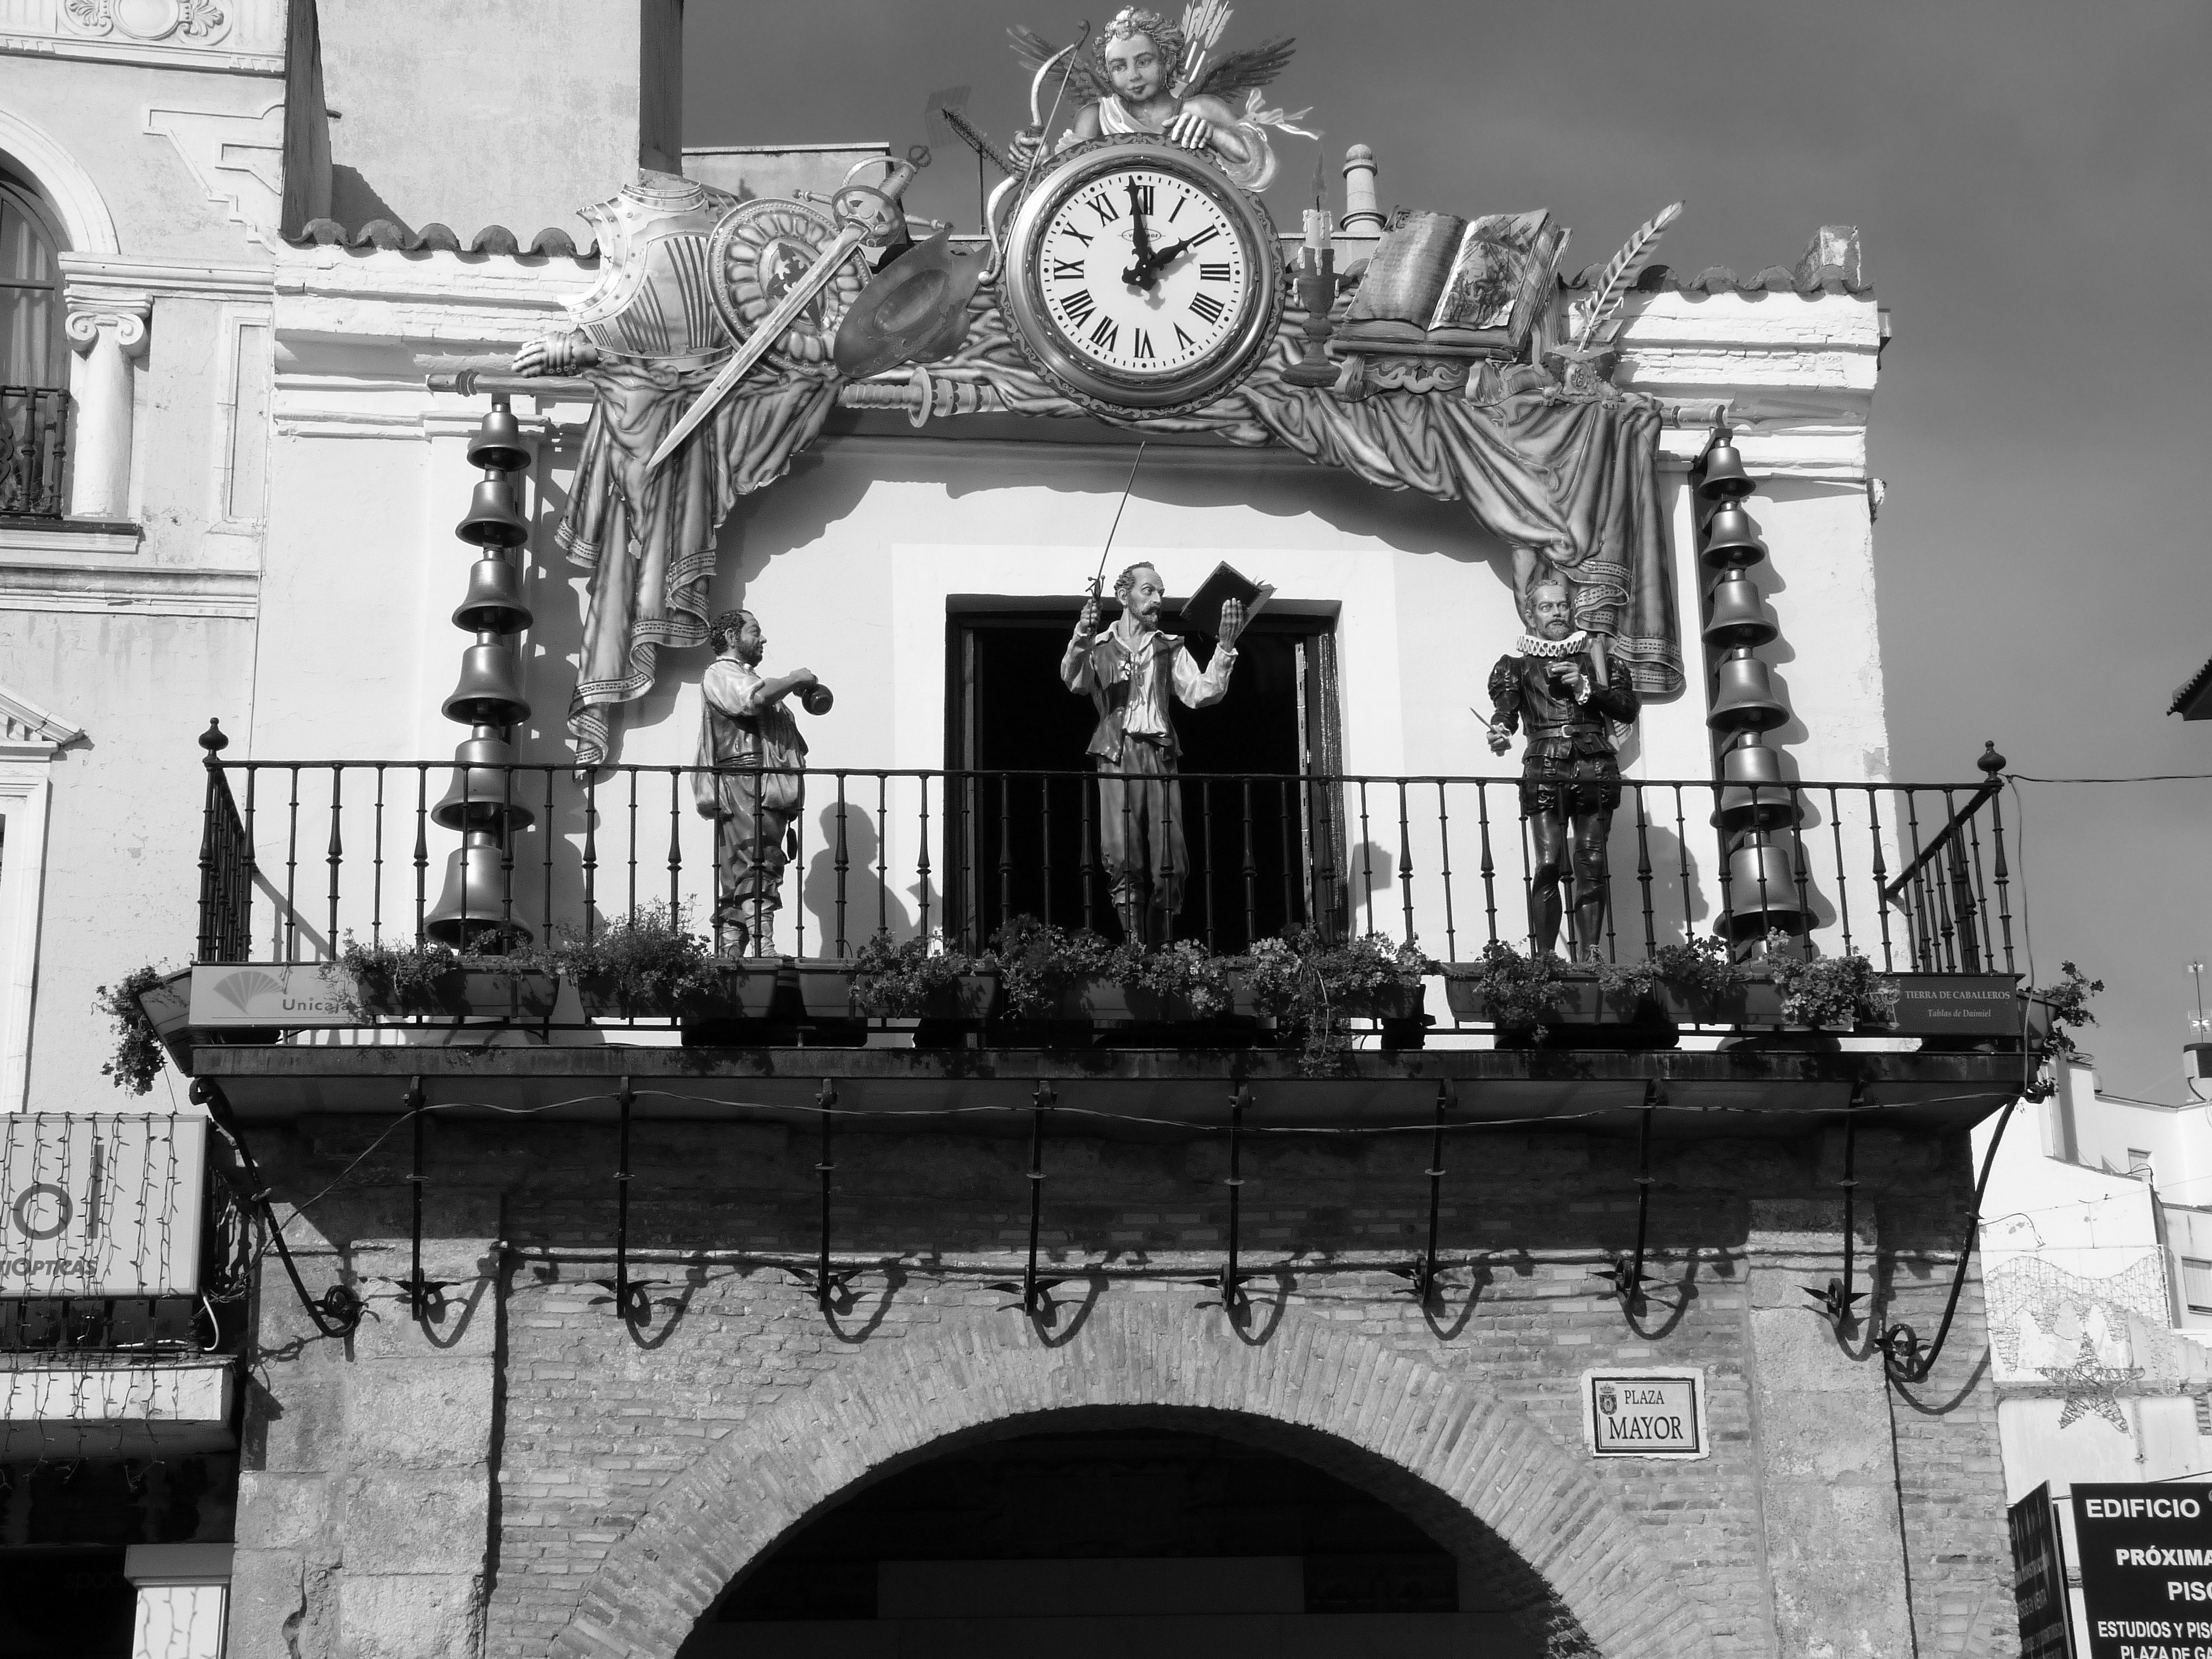
\includegraphics[width=0.8\linewidth]{./figs/clockCRbw}
		\caption{Fotografía en blanco y negro}\label{fig:fotoBW}
	\end{subfigure} 
	\caption[Ejemplo de subfiguras]{Ejemplo de inclusión de subfiguras en un mismo entorno (Fuente: J. Salido, \faCreativeCommons{} \faCreativeCommonsBy{} \faCreativeCommonsNcEu{} \faCreativeCommonsNd)}
	\label{fig:ejSubfigures}
\end{figure}

En los trabajos académicos la inclusión de imágenes y figuras que no son propiedad del autor suscitan bastante controversia. Ya que con frecuencia se incumple inadvertidamente la ley vigente de propiedad intelectual. Respecto a este hecho se recomienda, tanto a estudiantes como tutores, consultar documentación informativa sobre el uso correcto de figuras en documentos académicos \cite{uclm20,unican18}. Entre las <<incorrecciones>> más habituales en los documentos académicos, se observa:
\begin{itemize}
\item \emph{Abuso del derecho de cita}. Se produce al incluir, con fines exclusivamente decorativos o ilustrativos de la explicación, una figura sujeta a derechos de uso restringido invocando el derecho de cita (incluso con correcta atribución de la obra).

\item \emph{Incorrecta atribución de la obra}. Es habitual confundir al autor de la obra con la fuente de origen de la misma. La fuente es precisa cuando se cita la obra original. Sin embargo, la licencia de muchas obras exige la atribución al autor y la inclusión de la licencia bajo la que se distribuye o hace uso de la misma (véase como ejemplo cómo se realiza una correcta atribución en las Fig.~\ref{fig:ejFigure} y \ref{fig:ejSubfigures} mencionando al autor y la licencia Creative-Commons\footnote{\url{https://creativecommons.org}} bajo la que se rige el uso de la imagen y el mecanismo de título alternativo para que dicha atribución no aparezca en el índice de figuras usando título opcional).

\item \emph{Supresión de los detalles de la licencia de uso}. Al incluir obras de terceros debemos tener presente los términos de distribución de la misma e incluirlos junto a la atribución de su legítimo autor.
\end{itemize}

La inclusión de material de \emph{dominio público}, sin restricciones de uso o con permiso, hace innecesaria la atribución al autor, pero se recomienda incluir una nota de agradecimiento.\footnote{Incluyendo un texto como: \emph{<<Por cortesía de ...>>}}



\subsubsection{Algoritmos y listados de código fuente}
En los textos científicos relacionados con las 
TIC\footnote{Por supuesto, en un TFG (Trabajo Fin de Grado) o tesis 
de un centro superior de Informática.} (Tecnologías de la Información y 
Comunicaciones) suelen aparecer porciones de código en los que se explica 
alguna función o característica relevante del trabajo que se expone. Muchas 
veces lo que se quiere ilustrar es un algoritmo o método con el que se resuelve un problema abstrayéndose del lenguaje de implementación. El paquete \texttt{algorithm2e} proporciona un entorno \texttt{algorithm} para la impresión apropiada de algoritmos, tratándolos como objetos flotantes y con mucha flexibilidad de personalización, como se observa en el algoritmo~\ref{alg:como} del ejemplo.


% Ejemplo:
% ============
\IncMargin{1em}
\begin{algorithm}
\SetKwInOut{Input}{Datos}\SetKwInOut{Output}{Resultado}
\LinesNumbered
\SetAlgoLined

\Input{este texto} 
%\KwIn{este texto}
\Output{como escribir algoritmos con \LaTeX2e}
%\KwOut{como escribir algoritmos con \LaTeX2e}

inicialización\;
\While{no es el fin del documento}{
	leer actual\;
	\eIf{comprendido}{
		ir a la siguiente sección\;
		la sección actual es esta\;
	}{
		ir al principio de la sección actual\;
	}
}

% Aunque el captión aparece abajo siempre se pone arriba como en tablas y listados
\caption{Cómo escribir algoritmos}\label{alg:como}
\end{algorithm}\DecMargin{1em}








\newpage % Añadido para visualizar los listados completos en una página.
La inclusión de porciones de código fuente se puede formatear de modo sencillo en \LaTeX{} mediante el uso del paquete \texttt{listings}. A continuación, se muestran varios ejemplos de porciones de código correspondientes a distintos lenguajes de programación.


% Ejemplo: Listado Java
% ============
% Los entornos lstlisting se pueden tratar tambión como elementos flotantes mediante la opción 'float=hbt', donde se indica la ubicación del elemento.
\begin{lstlisting}[language=Java,caption={[Código fuente en Java]Ejemplo de código fuente en lenguaje Java},label=lst:java]
// @author www.javadb.com
public class Main {    
// Este método convierte un String a un vector de bytes

public void convertStringToByteArray() {

String stringToConvert = "This String is 15";      
	byte[] theByteArray = stringToConvert.getBytes();        
	System.out.println(theByteArray.length);        
}

public static void main(String[] args) {
	new Main().convertStringToByteArray();
}
}
\end{lstlisting}


\begin{lstlisting}[style=ruled,language=C,caption={Ejemplo de código fuente en lenguaje C},label=lst:codC]
// Este código se ha incluido tal cual está en el fichero \LaTeX{}
#include <stdio.h>

int main(int argc, char* argv[]) {
	puts("¡Hola mundo!");
}
\end{lstlisting}


\begin{lstlisting}[style=ruled,language=Matlab,caption={Ejemplo de script en Matlab},label=lst:matlab]
function f = fibonacci(n)
 % FIBONACCI  Fibonacci sequence
 %	f = FIBONACCI(n) generates the first n Fibonacci numbers.
 %	Copyright 2014 Cleve Moler
 %	Copyright 2014 The MathWorks, Inc.
f = zeros(n,1); 
f(1) = 1;
f(2) = 2;
for k = 3:n
f(k) = f(k-1) + f(k-2);
end
\end{lstlisting}



\subsubsection{Menús, paths y teclas con el paquete \texttt{menukeys}}
Cada vez es más usual que los trabajos en ingeniería exijan el uso de 
software. Para poder especificar de modo elegante el uso de menús, pulsación de 
teclas y directorios, se recomienda el uso del paquete 
\texttt{menukeys}.\footnote{\url{https://osl.ugr.es/CTAN/macros/latex/contrib/menukeys/menukeys.pdf}}
 \index{CTAN} Este paquete nos permite especificar el acceso a un menú, por 
ejemplo:\\

\noindent \menu{Herramientas:Órdenes:PDFLaTeX}\\

\noindent También un conjunto de teclas. Por ejemplo:
\keys{\ctrl + \shift + T}\\

\noindent O un directorio:
\directory{C:/user/LaTeX/Ejemplos}\\

\noindent Aunque este paquete permite muchas opciones de configuración de los estilos aplicados, no es necesario hacerlo para obtener unos resultados muy elegantes.


\subsection{Bibliografía}
Todo el material de terceros se debe citar convenientemente sin contravenir los términos de las licencias de uso y distribución de dicho material. Esto se extiende al uso de diagramas y fotografías. El incumplimiento de la legislación vigente en materia de protección de la propiedad intelectual es responsabilidad exclusiva del autor, independientemente de la cesión de derechos que este haya convenido.

La sección de \emph{Bibliografía}, que si se prefiere se puede titular \emph{Referencias}, incluirá un listado ordenado preferentemente por orden alfabético (primer apellido del autor principal), con todas las obras citadas en el texto. En la lista de referencias se especificará para cada obra: autores, título, editorial y año de publicación. Este formato se conseguirá en \LaTeX{} mediante el uso del estilo estándar \texttt{plain} o cualquier otro derivado con estilo de citación numérica. En algunas titulaciones se obliga a una ordenación por orden de cita en el texto que con Bib\TeX{} se puede obtener mediante los estilos estándar \texttt{ieeetr} (estilo para los IEEE \emph{transactions}) y \texttt{unsrt} (estilo \emph{unsorted}). 

Es muy importante tener presente que en esta sección solo se debe incluir las referencias bibliográficas citadas expresamente en el documento. Si se desea incluir fuentes consultadas, pero no citadas, se puede confeccionar con ellas una sección denominada \emph{Material de consulta}, aunque estas referencias se pueden incluir opcionalmente a lo largo del documento como notas a pie de página.

En las titulaciones técnicas se empleará estilo de citación numérico con el número de la referencia entre corchetes. La cita podrá incluir el número de página concreto de la referencia que se desea citar. El uso correcto de la citación implica dejar claro al lector cuál es el texto, material o idea citado. Las obras referenciadas sin mención explícita o implícita al material concreto citado se deberían considerar material de consulta y, por tanto, ser agrupadas como \emph{Material de consulta}, distinguiéndolas claramente de aquellas otras en las que si se recurre a la citación.

En las titulaciones que requieren un estilo de citación de tipo autor-año (no numérico), se puede incluir el paquete \LaTeX{} \texttt{apacite} (con la opción \texttt{natbibapa}) y especificar este mismo estilo en la sección de bibliografía en el argumento del comando \texttt{bibliographystyle}.

Cuando se desee incluir referencias a páginas genéricas de la Web sin mención expresa a un artículo con título y autor definido, dichas referencias se pueden incluir como notas al pie de página o como un apartado de fuentes de consulta dedicado a \emph{Direcciones de Internet}. Por el contrario, los documentos electrónicos publicados en Internet se pueden incluir empleando el tipo de entrada \texttt{misc} como se muestra en la bibliografía que acompaña esta plantilla.




